\documentclass[11pt,a4paper]{article}
\usepackage[utf8]{inputenc}
\usepackage[T1]{fontenc}
\usepackage[french]{babel}
\usepackage[margin=2.2cm]{geometry}
\usepackage{amsmath,amssymb,graphicx,booktabs,longtable,float,xcolor}
\usepackage[hidelinks]{hyperref}
\hypersetup{pdftitle={TP1 - Extraction, visualisation et cartographie 2D},pdfauthor={Houssam MAKHLOUK}}
\setlength{\parskip}{0.35em}
\graphicspath{{TP1_4_scans/resultats/}}
\title{TP -- Jour 1\\Extraction, visualisation et cartographie 2D\\\large Acquisition et fusion de quatre scans LD06}
\author{Houssam MAKHLOUK}
\date{3 novembre 2026}
\begin{document}
\hypersetup{pageanchor=false}
\begin{titlepage}
\thispagestyle{empty}
\centering
\vspace*{1.0cm}
{\Large\bfseries EIGSI\par}
\vspace{0.35cm}
{\large Ann\'ee universitaire 2026/2027\par}
\vspace{1.5cm}
{\large RAPPORT DE TRAVAUX PRATIQUES\par}
\vspace{0.4cm}
{\large Cartographie et localisation en robotique mobile\par}
\vspace{0.8cm}
{\color{blue!45!black}\rule{0.88\textwidth}{1.2pt}\par}
\vspace{0.6cm}
{\Huge\bfseries TP -- Jour 1\par}
\vspace{0.5cm}
{\LARGE\bfseries Extraction, visualisation\\[0.15cm]et cartographie 2D\par}
\vspace{0.65cm}
{\large Acquisition et fusion de quatre scans LiDAR LD06\par}
\vspace{0.6cm}
{\color{blue!45!black}\rule{0.88\textwidth}{1.2pt}\par}
\vfill
{\large R\'ealis\'e par\par}
\vspace{0.3cm}
{\LARGE\bfseries Houssam MAKHLOUK\par}
\vspace{0.3cm}
{\large \'Etudiant \`a EIGSI\par}
\vfill
{\large 3 novembre 2026\par}
\vspace*{0.6cm}
\end{titlepage}

\pagenumbering{roman}
\hypersetup{pageanchor=true}
\setcounter{tocdepth}{2}
\tableofcontents
\thispagestyle{plain}
\clearpage
\pagenumbering{arabic}

\begin{abstract}
Ce travail présente une chaîne de traitement de quatre acquisitions réelles du LiDAR LD06 : lecture de mesures polaires et cartésiennes, visualisation multi-scans, ajustement indépendant des poses, construction d'une carte d'occupation et d'une carte vectorielle. Le lot comprend 1\,821 mesures. La consolidation produit 38 segments et la grille comporte $288\times270$ cellules de 5 cm. Les poses sont estimées par recalage ; les résultats ne constituent pas une validation métrologique de la salle.
\end{abstract}

\section{Objectifs et données acquises}
Le TP demande de construire une représentation de l'environnement à partir de scans réels, puis de mettre à jour cette représentation lorsque de nouvelles observations sont disponibles. Deux formes complémentaires sont réalisées : une grille d'occupation et une liste de segments.

\subsection{Capteur et acquisition}
Les deux acquisitions récentes ont été enregistrées par liaison USB via une carte ESP32, sur le port COM3 à 115\,200 bauds. Ce débit concerne la sortie CSV de l'ESP32 vers le PC, et non nécessairement la liaison interne du capteur. Les messages de démarrage et les lignes incomplètes sont écartés. Un tour est retenu lorsque ses indices sont consécutifs et que sa couverture angulaire est supérieure ou égale à $350^\circ$. Ce contrôle n'atteste pas à lui seul l'absence de mouvement ni la précision du montage.

\begin{table}[H]\centering
\begin{tabular}{lrl}
\toprule Scan & Nombre de points & Hauteur déclarée \\
\midrule
1 & 454 & 1,90 m \\
2 & 454 & 1,90 m \\
3 & 456 & 1,90 m \\
4 & 457 & 1,90 m \\
\midrule Total & 1\,821 & \\
\bottomrule
\end{tabular}
\caption{Jeux de données utilisés. La hauteur de 1,90 m pour les quatre scans est une déclaration de l'utilisateur lors de la préparation de ce rapport ; elle n'est pas mesurée par le LiDAR. Aucune incertitude chiffrée de hauteur n'a été fournie.}
\end{table}
Les données originales sont conservées dans \path{TP1_4_scans/data/}. Chaque fichier contient l'indice, l'angle en degrés, la distance en millimètres, l'intensité et les coordonnées cartésiennes locales. Les conditions détaillées de la liaison série des deux acquisitions anciennes ne sont pas documentées.

\section{Repères, conversion et visualisation}
Dans un repère polaire mathématique usuel, $x=r\cos\alpha$ et $y=r\sin\alpha$. Les CSV employés suivent la convention $y\simeq-r\sin\alpha$. Le traitement conserve les coordonnées cartésiennes fournies et convertit les millimètres en mètres, sans inverser une seconde fois l'axe $Y$.
Pour une pose $\mathbf{q}=(x_r,y_r,\theta_r)$, un point local est placé dans la carte par :
\[
 \mathbf p_g=\underbrace{\begin{bmatrix}\cos\theta_r&-\sin\theta_r\\\sin\theta_r&\cos\theta_r\end{bmatrix}}_{R(\theta_r)}\mathbf p_l+\begin{bmatrix}x_r\\y_r\end{bmatrix}.
\]
Le viewer affiche les quatre nuages avec quatre couleurs. Le choix d'un scan active ses curseurs $X$, $Y$ et $\theta$ ; sa pose peut ainsi être ajustée sans déplacer les autres scans. Les poses se sauvegardent dans un fichier JSON. Les cartes sont reconstruites depuis les sources lorsqu'un curseur change pour éviter de conserver des traces d'une ancienne pose.
Cette visualisation est la première vérification du traitement : deux acquisitions qui voient le même mur doivent dessiner des lignes proches après transformation. Une séparation persistante entre ces lignes peut venir d'une mauvaise pose, d'une surface observée différemment ou d'un obstacle mobile. Le graphique sert donc à diagnostiquer le recalage avant de construire les cartes ; il ne fournit pas, à lui seul, la pose vraie du LiDAR.

\subsection{Recalage estimé des quatre acquisitions}
Le scan 3 définit l'origine du repère global. Une recherche multi-départs initialise un ICP robuste : 36 rotations espacées de $10^\circ$, neuf décalages de translation par rotation, puis raffinement des meilleurs candidats. À chaque itération, 65\,\% des correspondances les plus proches servent à estimer une rotation et une translation par SVD. Le choix final utilise une distance symétrique plafonnée à 0,40 m.
La rotation est libre : une hypothèse antérieure d'orientation identique donnait une superposition insuffisante.

\begin{table}[H]\centering
\begin{tabular}{lrrr}\toprule Scan & $x_r$ (m) & $y_r$ (m) & $\theta_r$ ($^\circ$) \\
\midrule
1 & 2,789 & 1,193 & 174,051 \\
2 & 5,603 & $-1,342$ & $-83,932$ \\
3 & 0 & 0 & 0 \\
4 & 0,041 & $-0,010$ & $-90,057$ \\
\bottomrule\end{tabular}
\caption{Poses estimées, non mesurées sur le terrain. Le scan 4 semble essentiellement tourné par rapport au scan 3 ; cette interprétation reste à confirmer.}
\end{table}
\begin{figure}[H]\centering
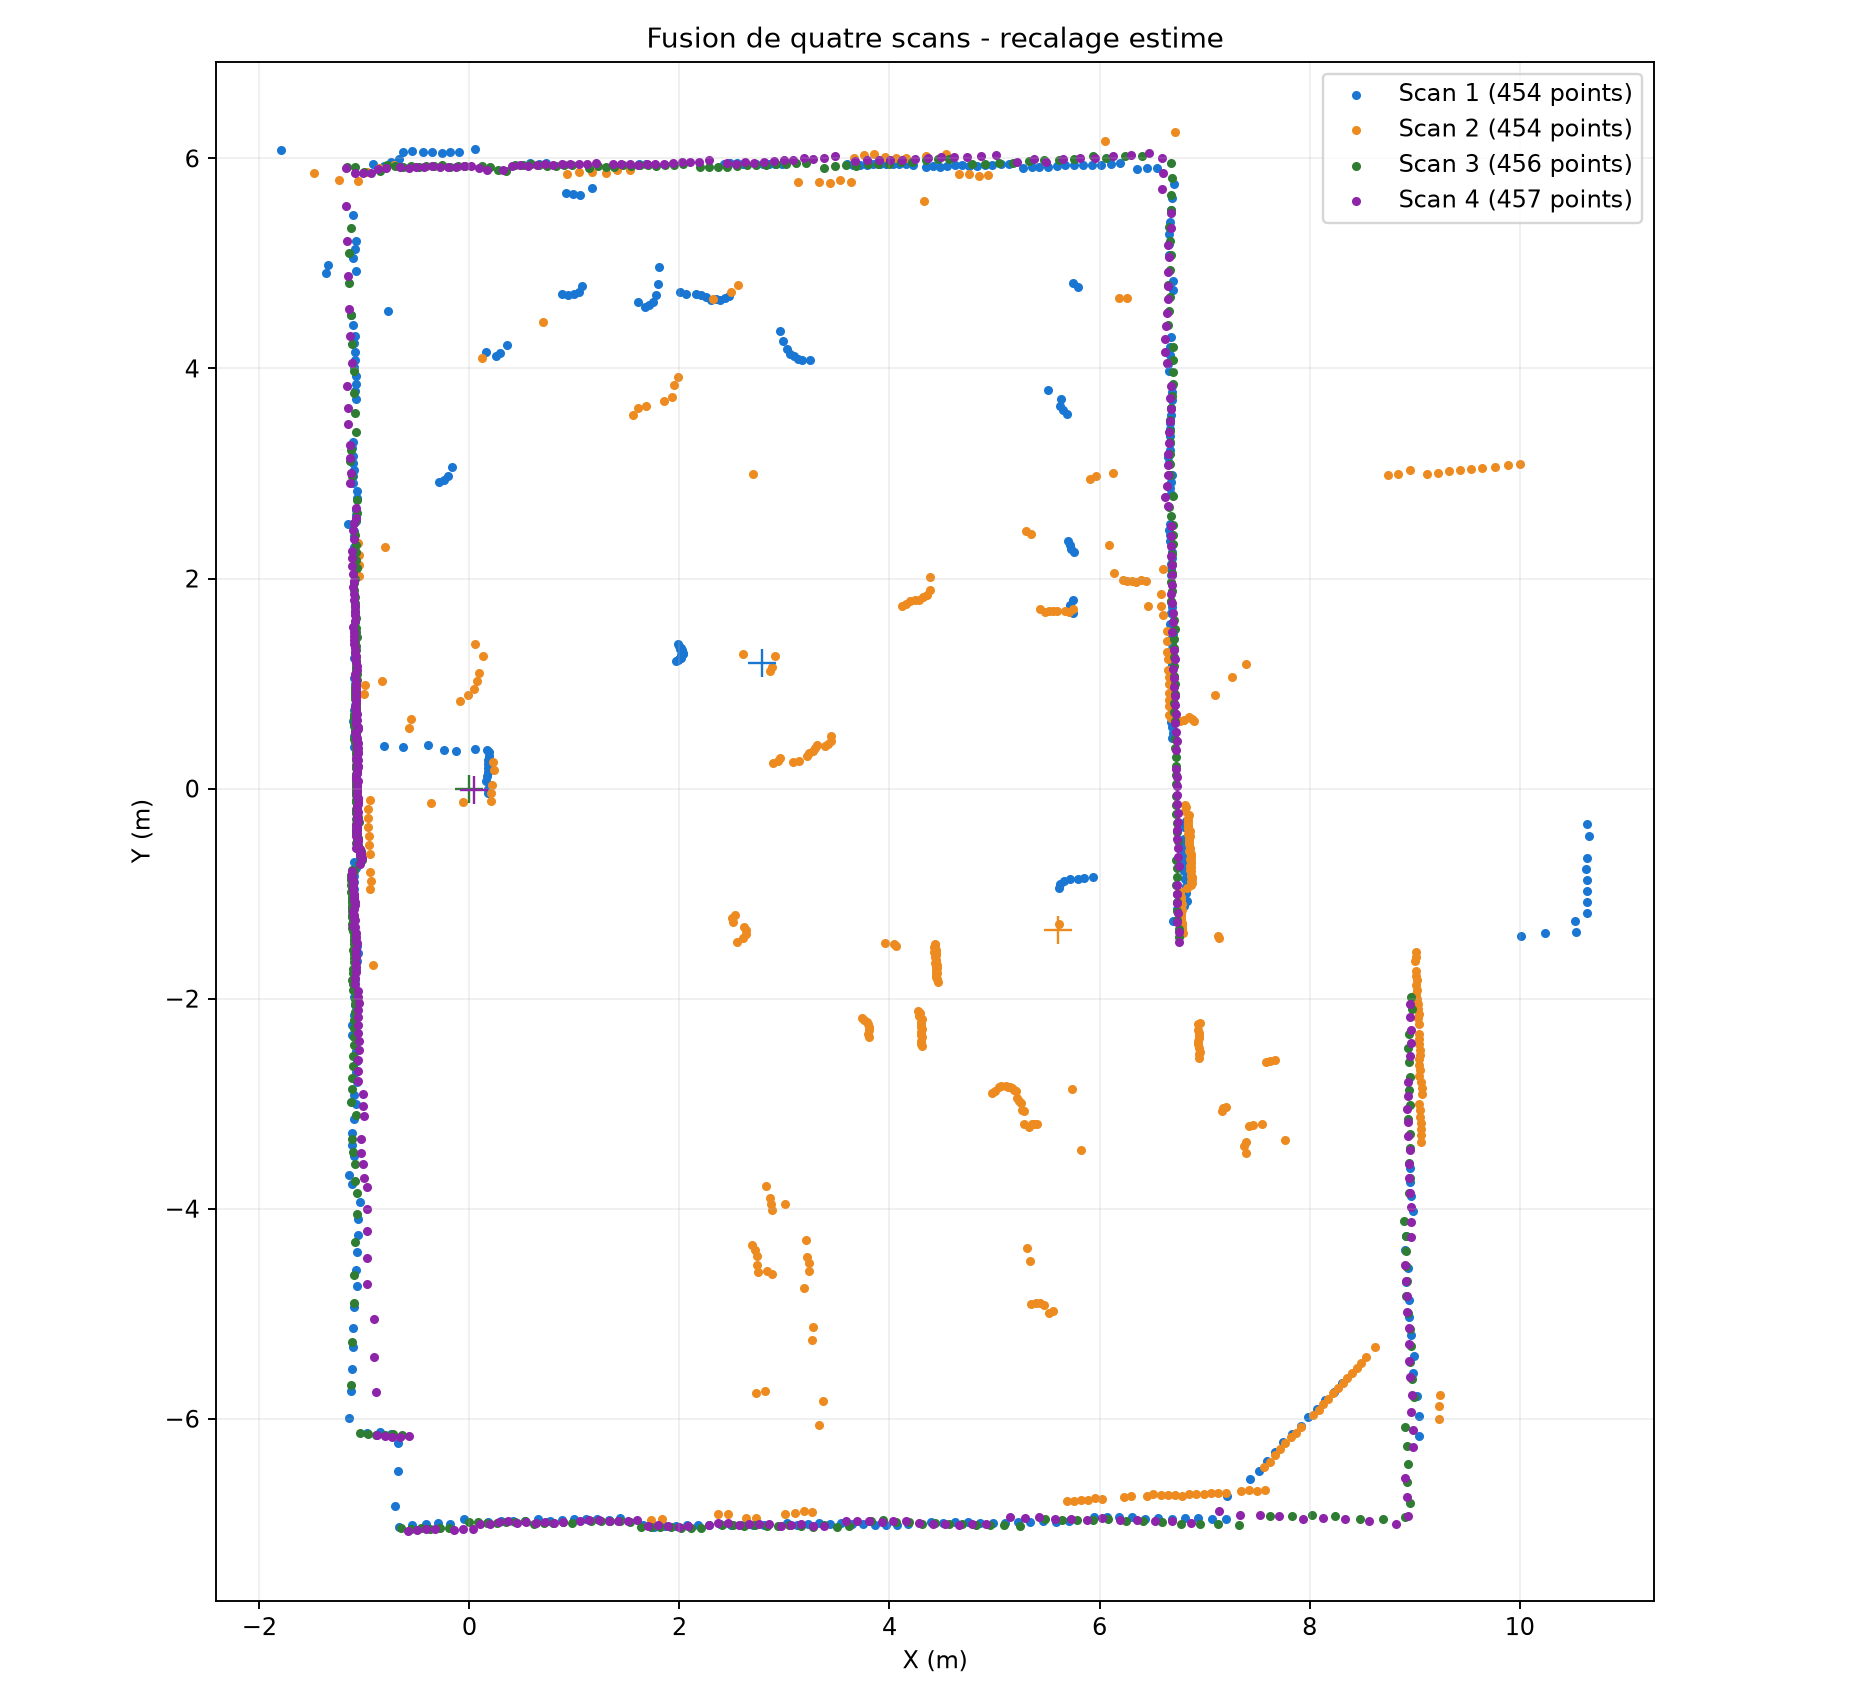
\includegraphics[width=.83\linewidth,height=.64\textheight,keepaspectratio]{fusion_4_scans.png}
\caption{Superposition des quatre nuages dans le repère du scan 3. Les croix indiquent les origines estimées des capteurs.}
\end{figure}

\subsection{Indicateurs de cohérence}
\begin{table}[H]\centering
\begin{tabular}{lrrr}\toprule Scan vers référence 3 & Voisins à moins de 20 cm & Score plafonné (m) & Calcul (s) \\
\midrule
1 & 72,2\,\% & 0,191 & 11,99 \\
2 & 37,3\,\% & 0,301 & 11,52 \\
4 & 99,1\,\% & 0,050 & 11,26 \\
\bottomrule\end{tabular}
\caption{Mesures du calcul enregistré dans \texttt{alignement.json}. Les temps dépendent du poste et de sa charge. Le score est la racine de la moyenne symétrique des distances au carré plafonnées, et non une erreur de pose.}
\end{table}
Les nouveaux scans se correspondent très bien sur les surfaces observées. Le scan 1 se superpose partiellement ; le scan 2 reste moins fiable. Une proportion faible peut refléter des occultations, des objets déplacés, des différences de scène ou un mauvais recalage. Sans positions de référence mesurées, on ne peut pas convertir ces indicateurs en précision réelle de localisation.

\subsection{Dimensions visibles estimées depuis les CSV}
Les scans 3 et 4, dont les impacts se superposent à environ 99\,\% à moins de
20 cm, servent à décrire l'emprise principale observée sans les extensions
isolées du scan 2. Les bornes des points alignés sont $x\in[-1{,}18;9{,}00]$ m
et $y\in[-7{,}06;6{,}05]$ m, soit environ \textbf{10,17 m selon X et
13,11 m selon Y}. Le calcul est enregistré dans
\texttt{resultats/dimensions\_estimees.json} et reproduit par
\texttt{generer.py}. Ces valeurs sont l'emprise des impacts visibles au niveau
du LiDAR, et non une mesure indépendante de la longueur et de la largeur des
murs : occultations, ouvertures et erreurs de recalage peuvent modifier les
limites observées. Les dimensions de la grille, qui incluent une marge et les
quatre scans, ne doivent pas être interprétées comme celles de la salle.

\section{Construction et mise à jour de la carte d'occupation}
\subsection{Structure et indices}
La grille est initialement inconnue. Sa résolution est $\rho=0{,}05$ m ; son emprise couvre les points valides transformés et les origines des capteurs, avec une marge de 0,50 m. Elle contient 288 lignes et 270 colonnes, soit 77\,760 cellules. Le stockage est un tableau \texttt{int16}, soit 155\,520 octets pour les états seuls.
\begin{center}\begin{tabular}{lll}\toprule Valeur & État & Couleur \\
\midrule $-1$ & Inconnu & Marron \\ 0 & Libre & Vert \\ 100 & Occupé & Rouge \\
\bottomrule\end{tabular}\end{center}
Ces trois valeurs sont des états discrets, pas des probabilités. Les positions des capteurs sont bleues. Pour une origine de grille $(x_{\min},y_{\min})$ :
\[
 c=\left\lfloor\frac{x-x_{\min}}{\rho}\right\rfloor,\qquad
 l=\left\lfloor\frac{y-y_{\min}}{\rho}\right\rfloor.
\]
L'arrondi inférieur évite une erreur d'indice pour les coordonnées négatives. La ligne 0 du CSV correspond au plus petit $Y$.

\subsection{Traitement d'un scan et mises à jour}
\begin{enumerate}
\item Écarter les points non finis et ceux dont la portée locale est hors de $[0{,}15;12]$ m. L'intensité est conservée dans les données, mais aucun seuil de qualité non calibré n'est imposé.
\item Transformer les points selon la pose du scan et calculer les indices des cellules.
\item Tracer chaque rayon depuis le capteur jusqu'à l'impact par Bresenham.
\item Marquer libres les cellules avant l'impact et occupée la cellule d'impact.
\item Accumuler les cellules puis donner priorité aux impacts au sein d'un même scan, afin que l'ordre des faisceaux ne modifie pas le résultat.
\end{enumerate}
Les scans 1, 2, 3 puis 4 mettent à jour le même objet. Une nouvelle observation remplace l'ancien état uniquement dans les cellules touchées ; les autres restent inchangées. Un obstacle ancien traversé par un nouveau rayon peut ainsi redevenir libre. Une carte NPZ peut être rechargée par \texttt{GridMap.load}, puis mise à jour par \texttt{update(scan, pose)}.

\begin{figure}[H]\centering
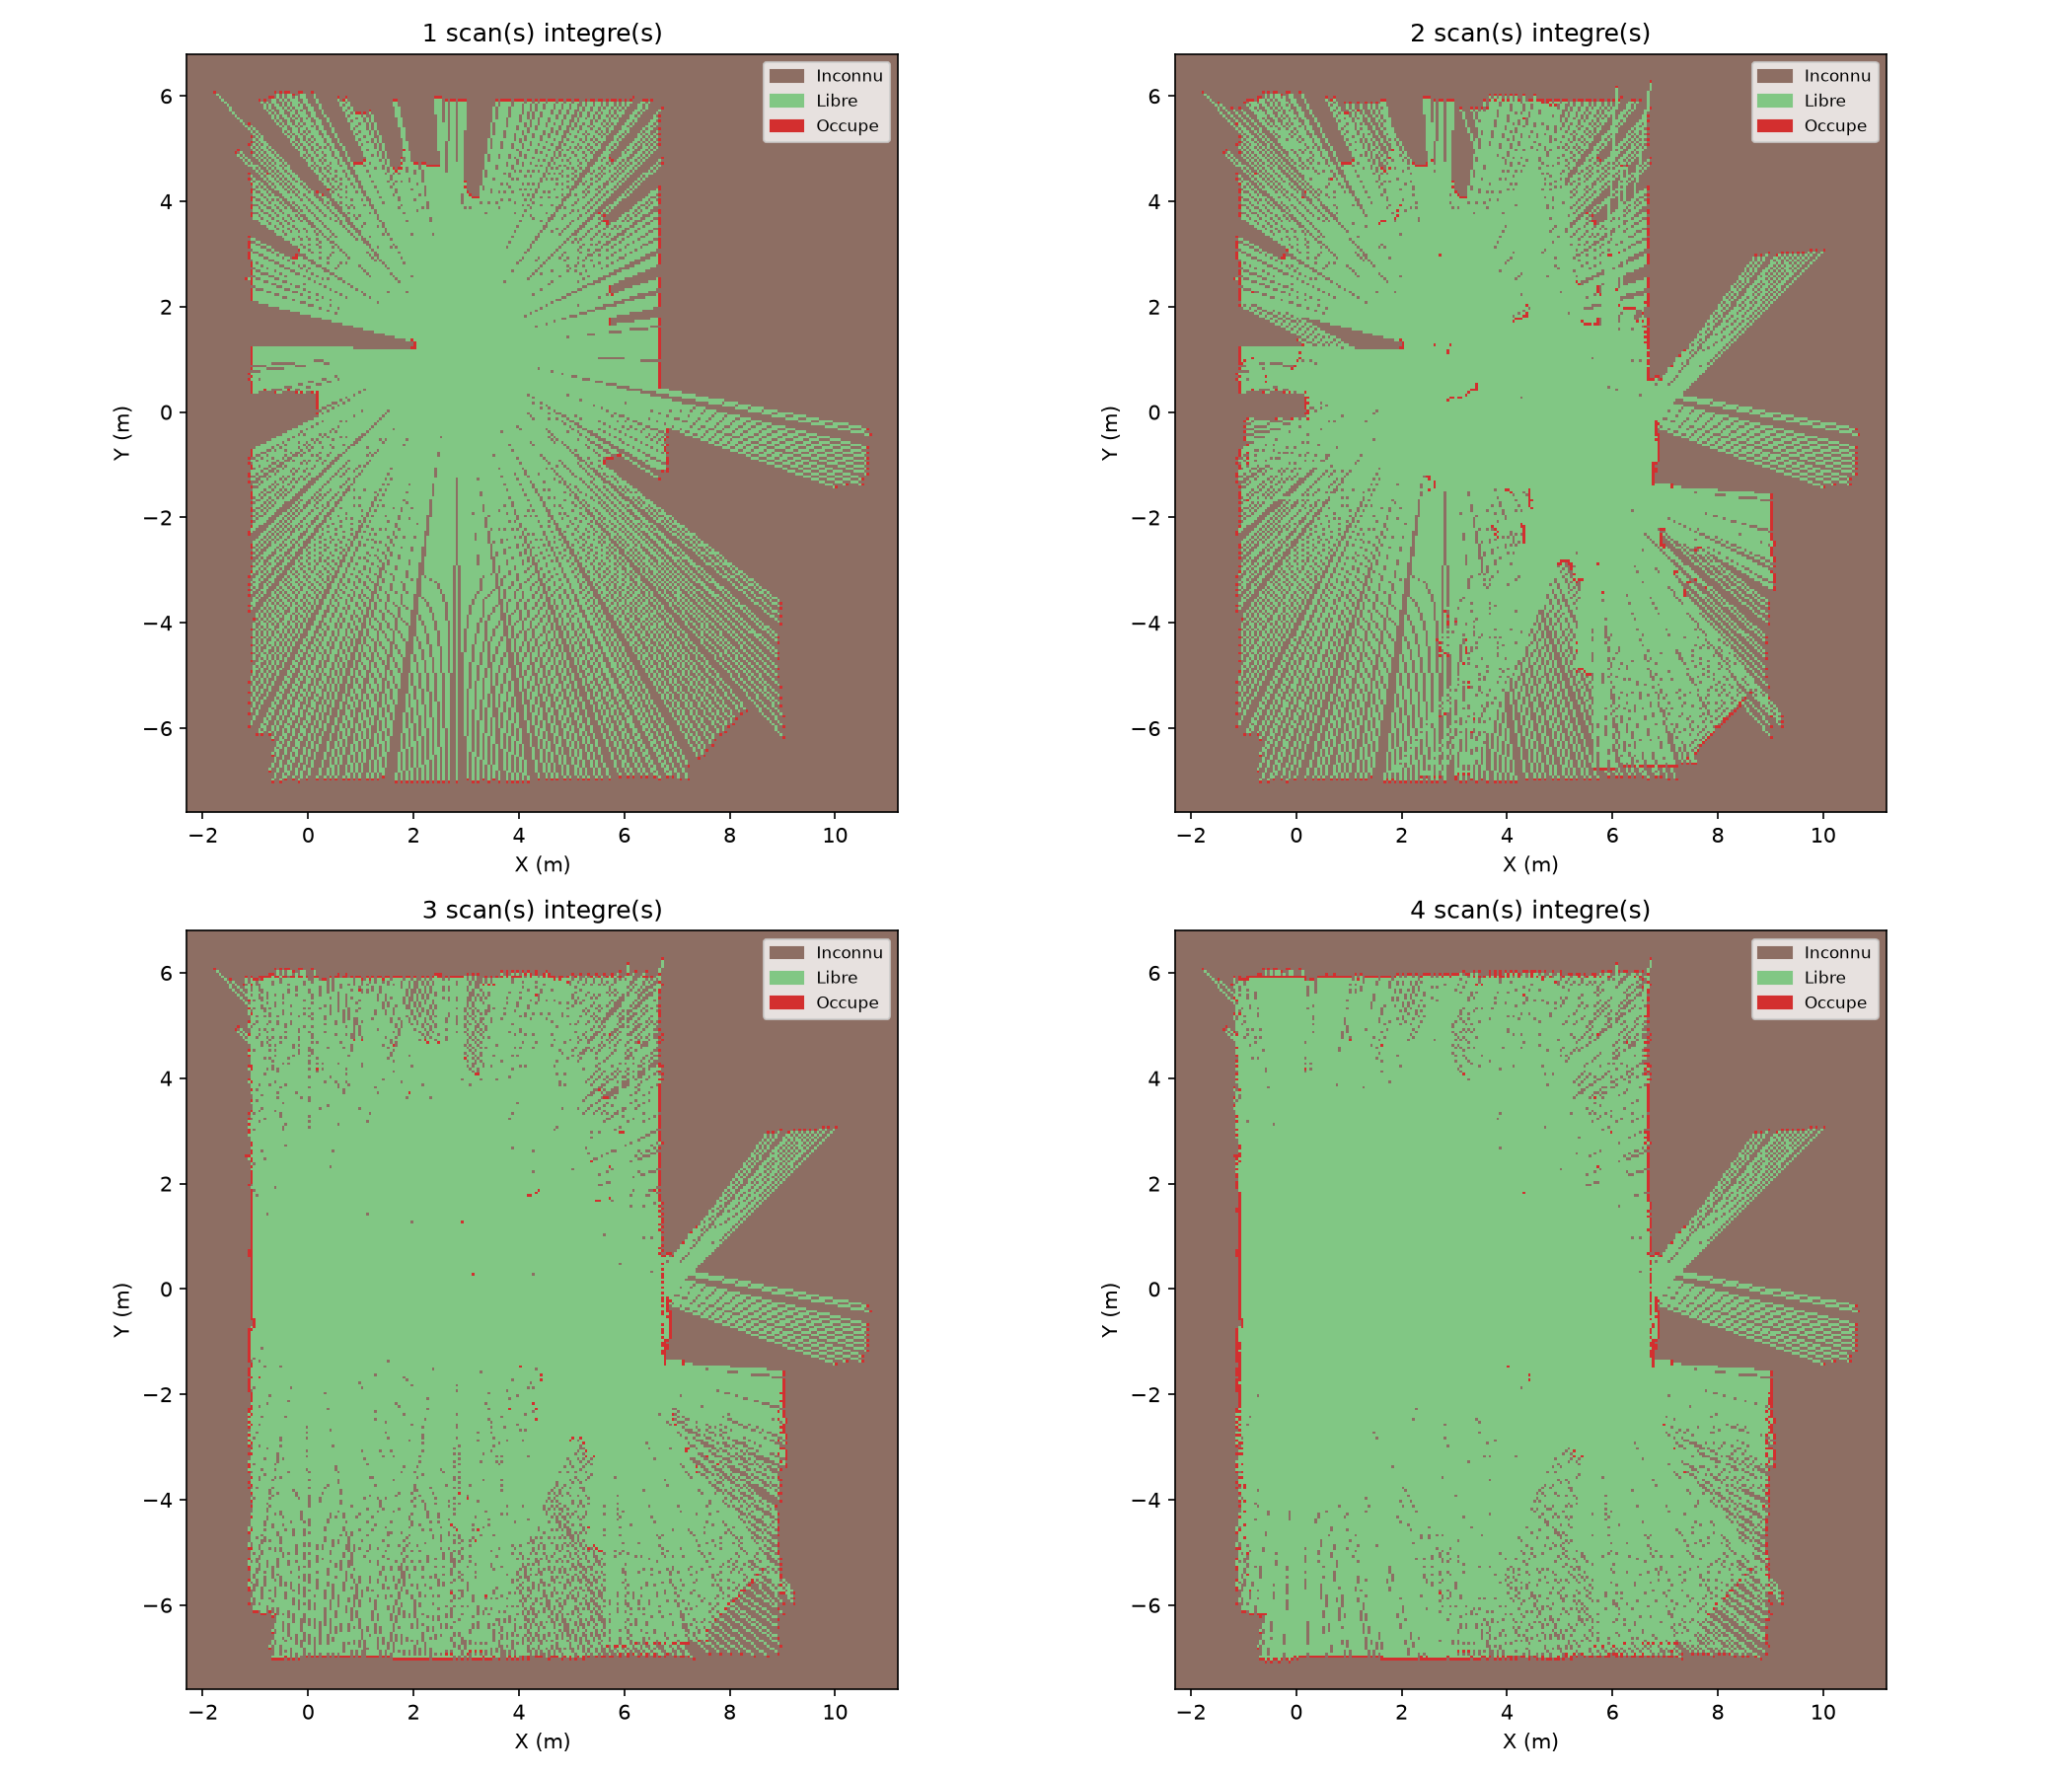
\includegraphics[width=\linewidth,height=.65\textheight,keepaspectratio]{grid_map_progression.png}
\caption{Évolution cumulative de la même grille après chaque scan.}
\end{figure}
\begin{figure}[H]\centering
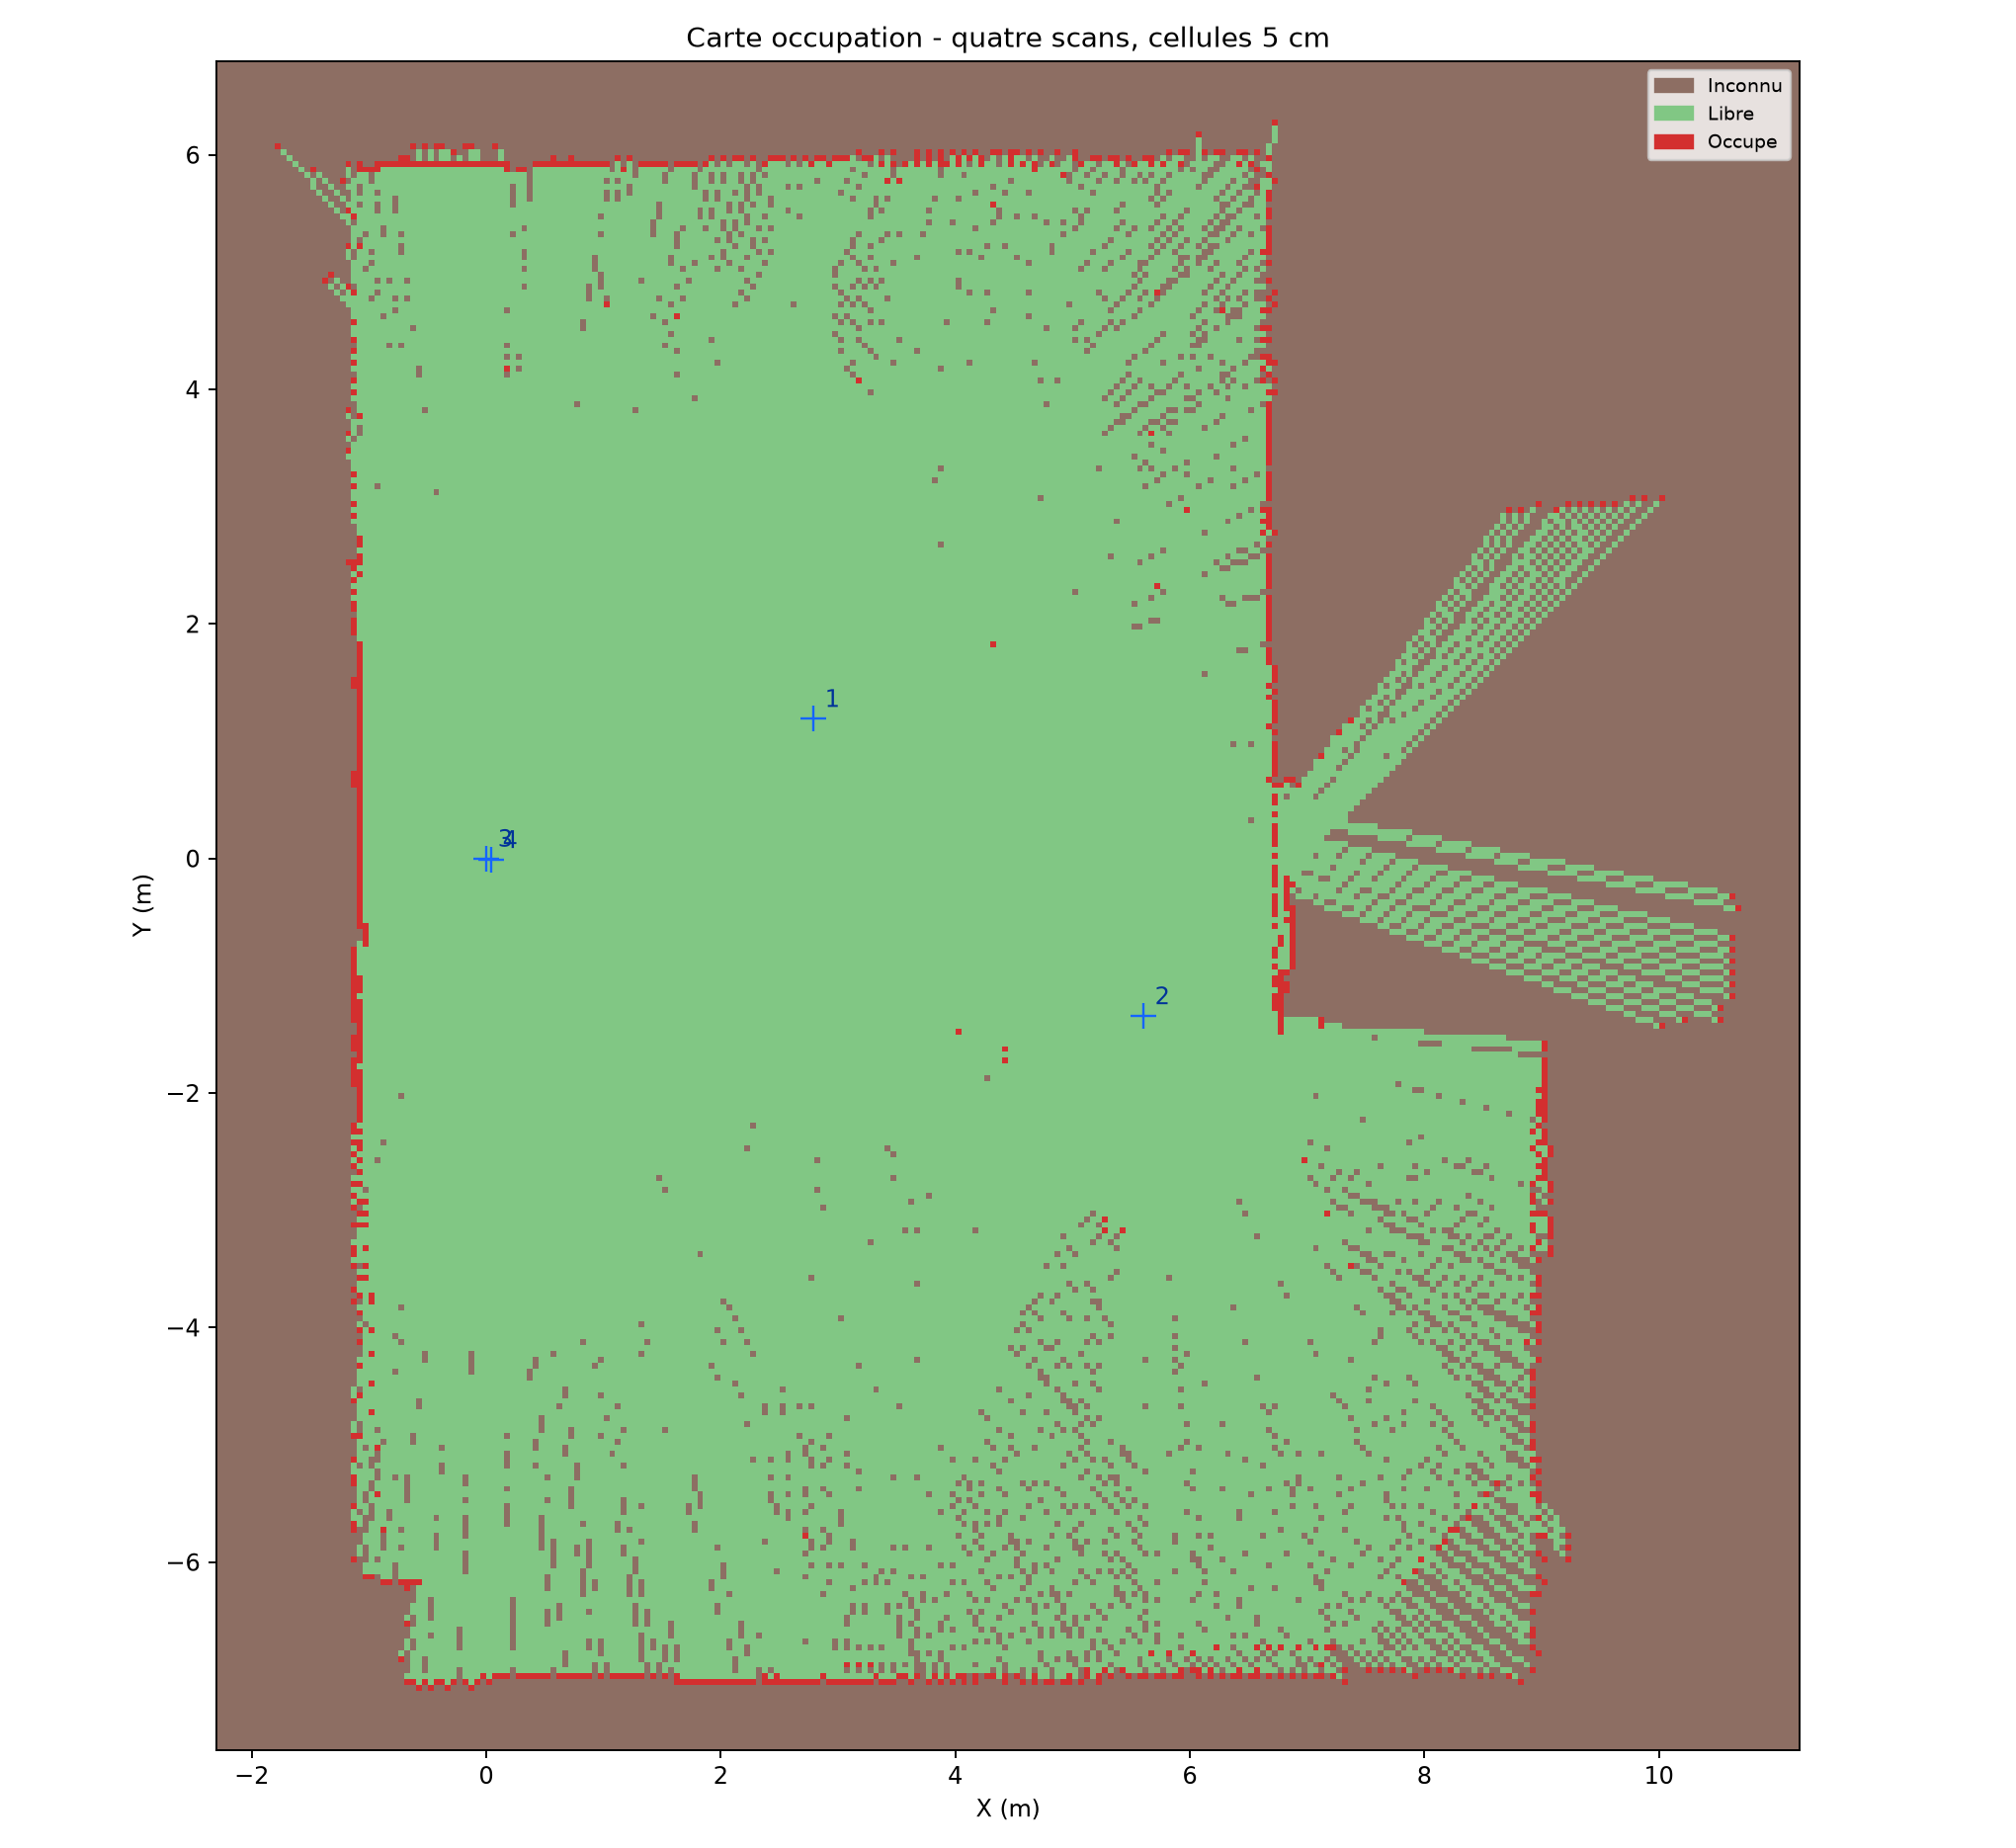
\includegraphics[width=.88\linewidth,height=.7\textheight,keepaspectratio]{grid_map_finale.png}
\caption{Carte d'occupation fusionnée. Les cellules entre deux faisceaux restent inconnues lorsqu'aucun rayon ne les a traversées.}
\end{figure}
\begin{figure}[H]\centering
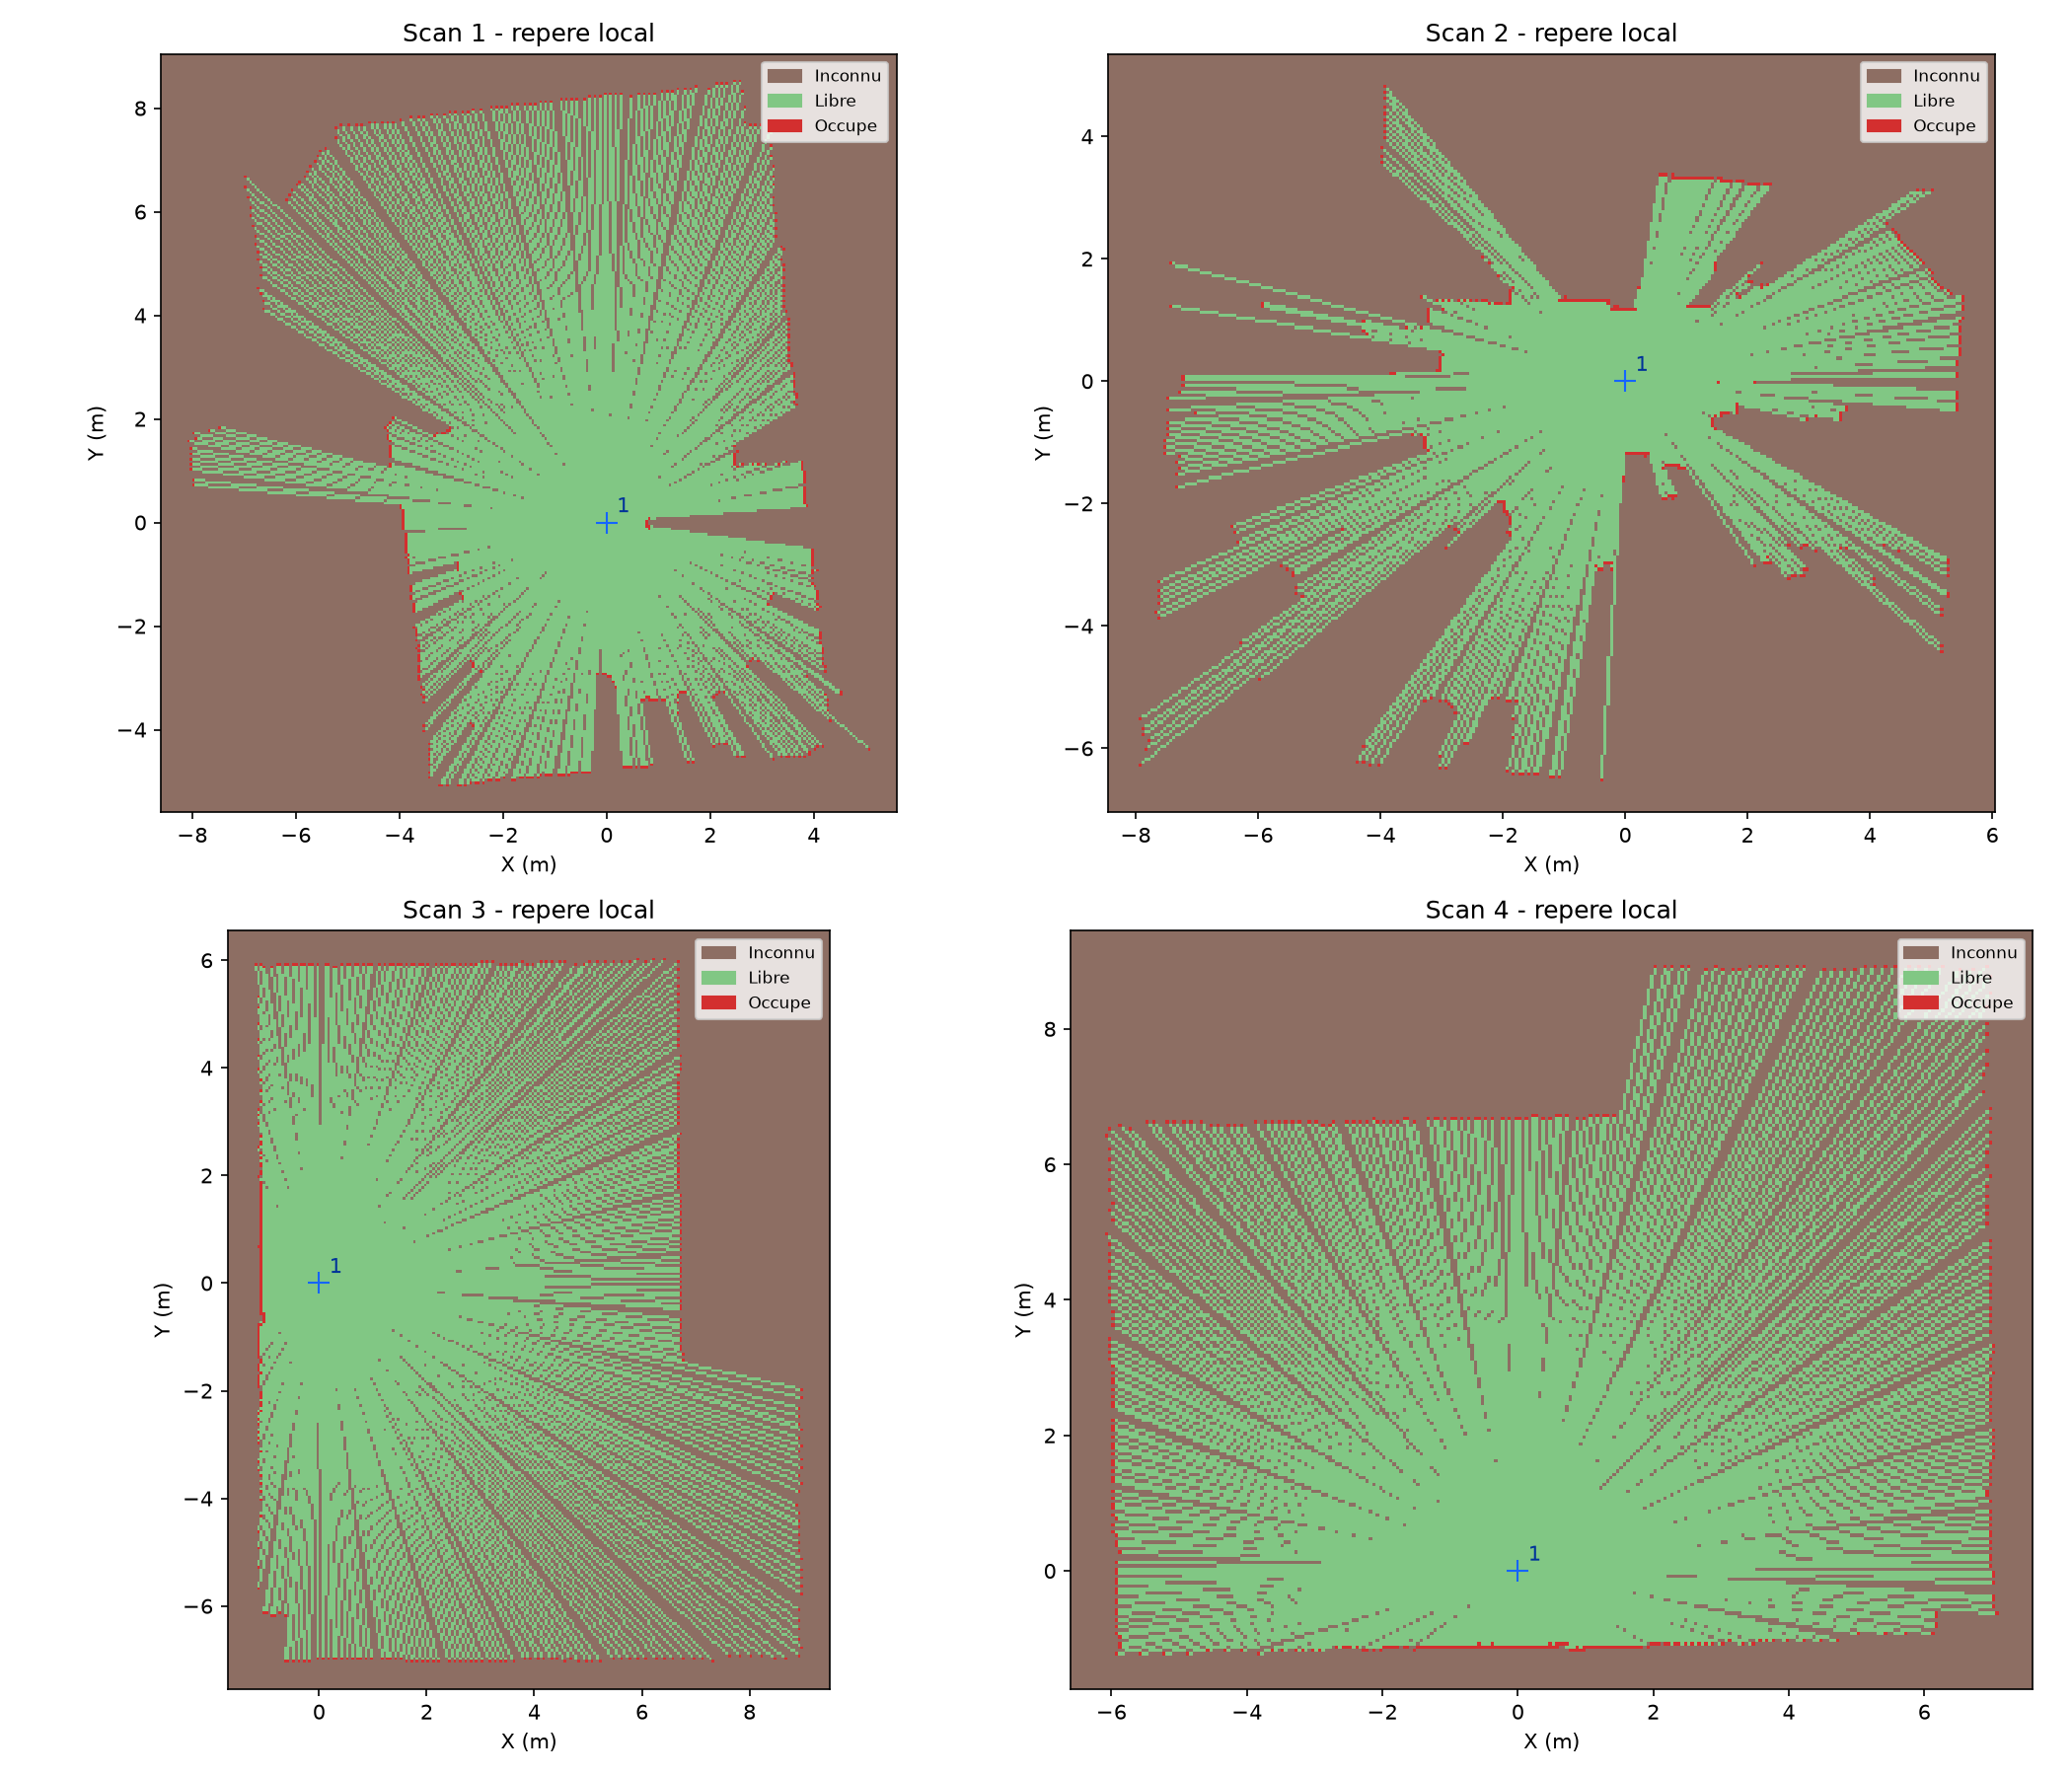
\includegraphics[width=\linewidth,height=.65\textheight,keepaspectratio]{grilles_individuelles.png}
\caption{Cartes d'occupation individuelles dans les repères locaux des quatre acquisitions. Elles ne partagent pas une origine commune.}
\end{figure}

\section{Extraction et manipulation des segments}
\subsection{Extraction}
Les points sont regroupés selon l'ordre d'acquisition ; une distance supérieure à 0,32 m entre voisins ou une mesure invalide interrompt le groupe. Un ajustement de droite par PCA/SVD est appliqué. Si l'erreur perpendiculaire maximale dépasse 0,06 m, le groupe est divisé selon sa géométrie, puis réajusté récursivement. Un segment nécessite au moins cinq points et une longueur minimale de 0,20 m. Les courbes et les petits objets peuvent donc être simplifiés ou rejetés.

\subsection{Opérations implémentées}
L'angle non orienté entre deux directions $\mathbf u,\mathbf v$ est :
\[
 \beta=\arccos\!\left(\frac{|\mathbf u\cdot\mathbf v|}{\|\mathbf u\|\|\mathbf v\|}\right).
\]
Deux segments sont proches si leur angle est au plus $8^\circ$, leur écart de droite support aux milieux au plus 0,15 m et leur séparation projetée au plus 0,25 m. Leur fusion ajuste une droite sur les quatre extrémités et conserve les extrêmes projetés.
L'intersection résout les paramètres des deux segments ; elle n'est acceptée que si elle appartient aux deux. Les segments parallèles ou colinéaires ne fournissent pas d'intersection unique pour cette opération.

Pour le découpage demandé :
\begin{itemize}
\item l'intersection doit être strictement intérieure au segment à couper ;
\item une intersection à son extrémité ne le modifie pas ;
\item les segments colinéaires ne sont pas découpés ;
\item le côté le plus long est conservé ; en cas d'égalité à la tolérance près, on garde celui contenant le premier point.
\end{itemize}
La tolérance spatiale est $\varepsilon=10^{-8}$ m ; elle est convertie en tolérance paramétrique selon la longueur. Le seuil relatif de parallélisme est $10^{-12}$. Des tests couvrent les extrémités, les intersections hors des segments, la colinéarité, les segments dégénérés et les longueurs égales.

\section{Carte vectorielle et consolidation}
Chaque primitive est stockée par ses deux extrémités, un compteur d'associations et l'indice du dernier scan associé. Les primitives extraites localement sont transformées dans le repère global puis comparées à celles de la carte. Une primitive similaire est fusionnée ; sinon elle est ajoutée. La consolidation est répétée si une fusion rend possible une nouvelle association. Les quatre acquisitions produisent finalement 38 segments consolidés.
Le compteur comptabilise les primitives associées ; ce n'est ni une probabilité ni nécessairement le nombre de scans distincts.

Le mode général permet de découper les anciens segments traversés par de nouveaux rayons, raccourcis de 0,15 m avant l'impact. Pour la fusion présentée, cet effacement est désactivé par prudence face aux erreurs de pose et aux changements de scène. Il reste disponible et testé dans \texttt{VectorMap.update}. Le viewer reproduit ce choix avec \texttt{--keep-vector-features}.

\begin{figure}[H]\centering
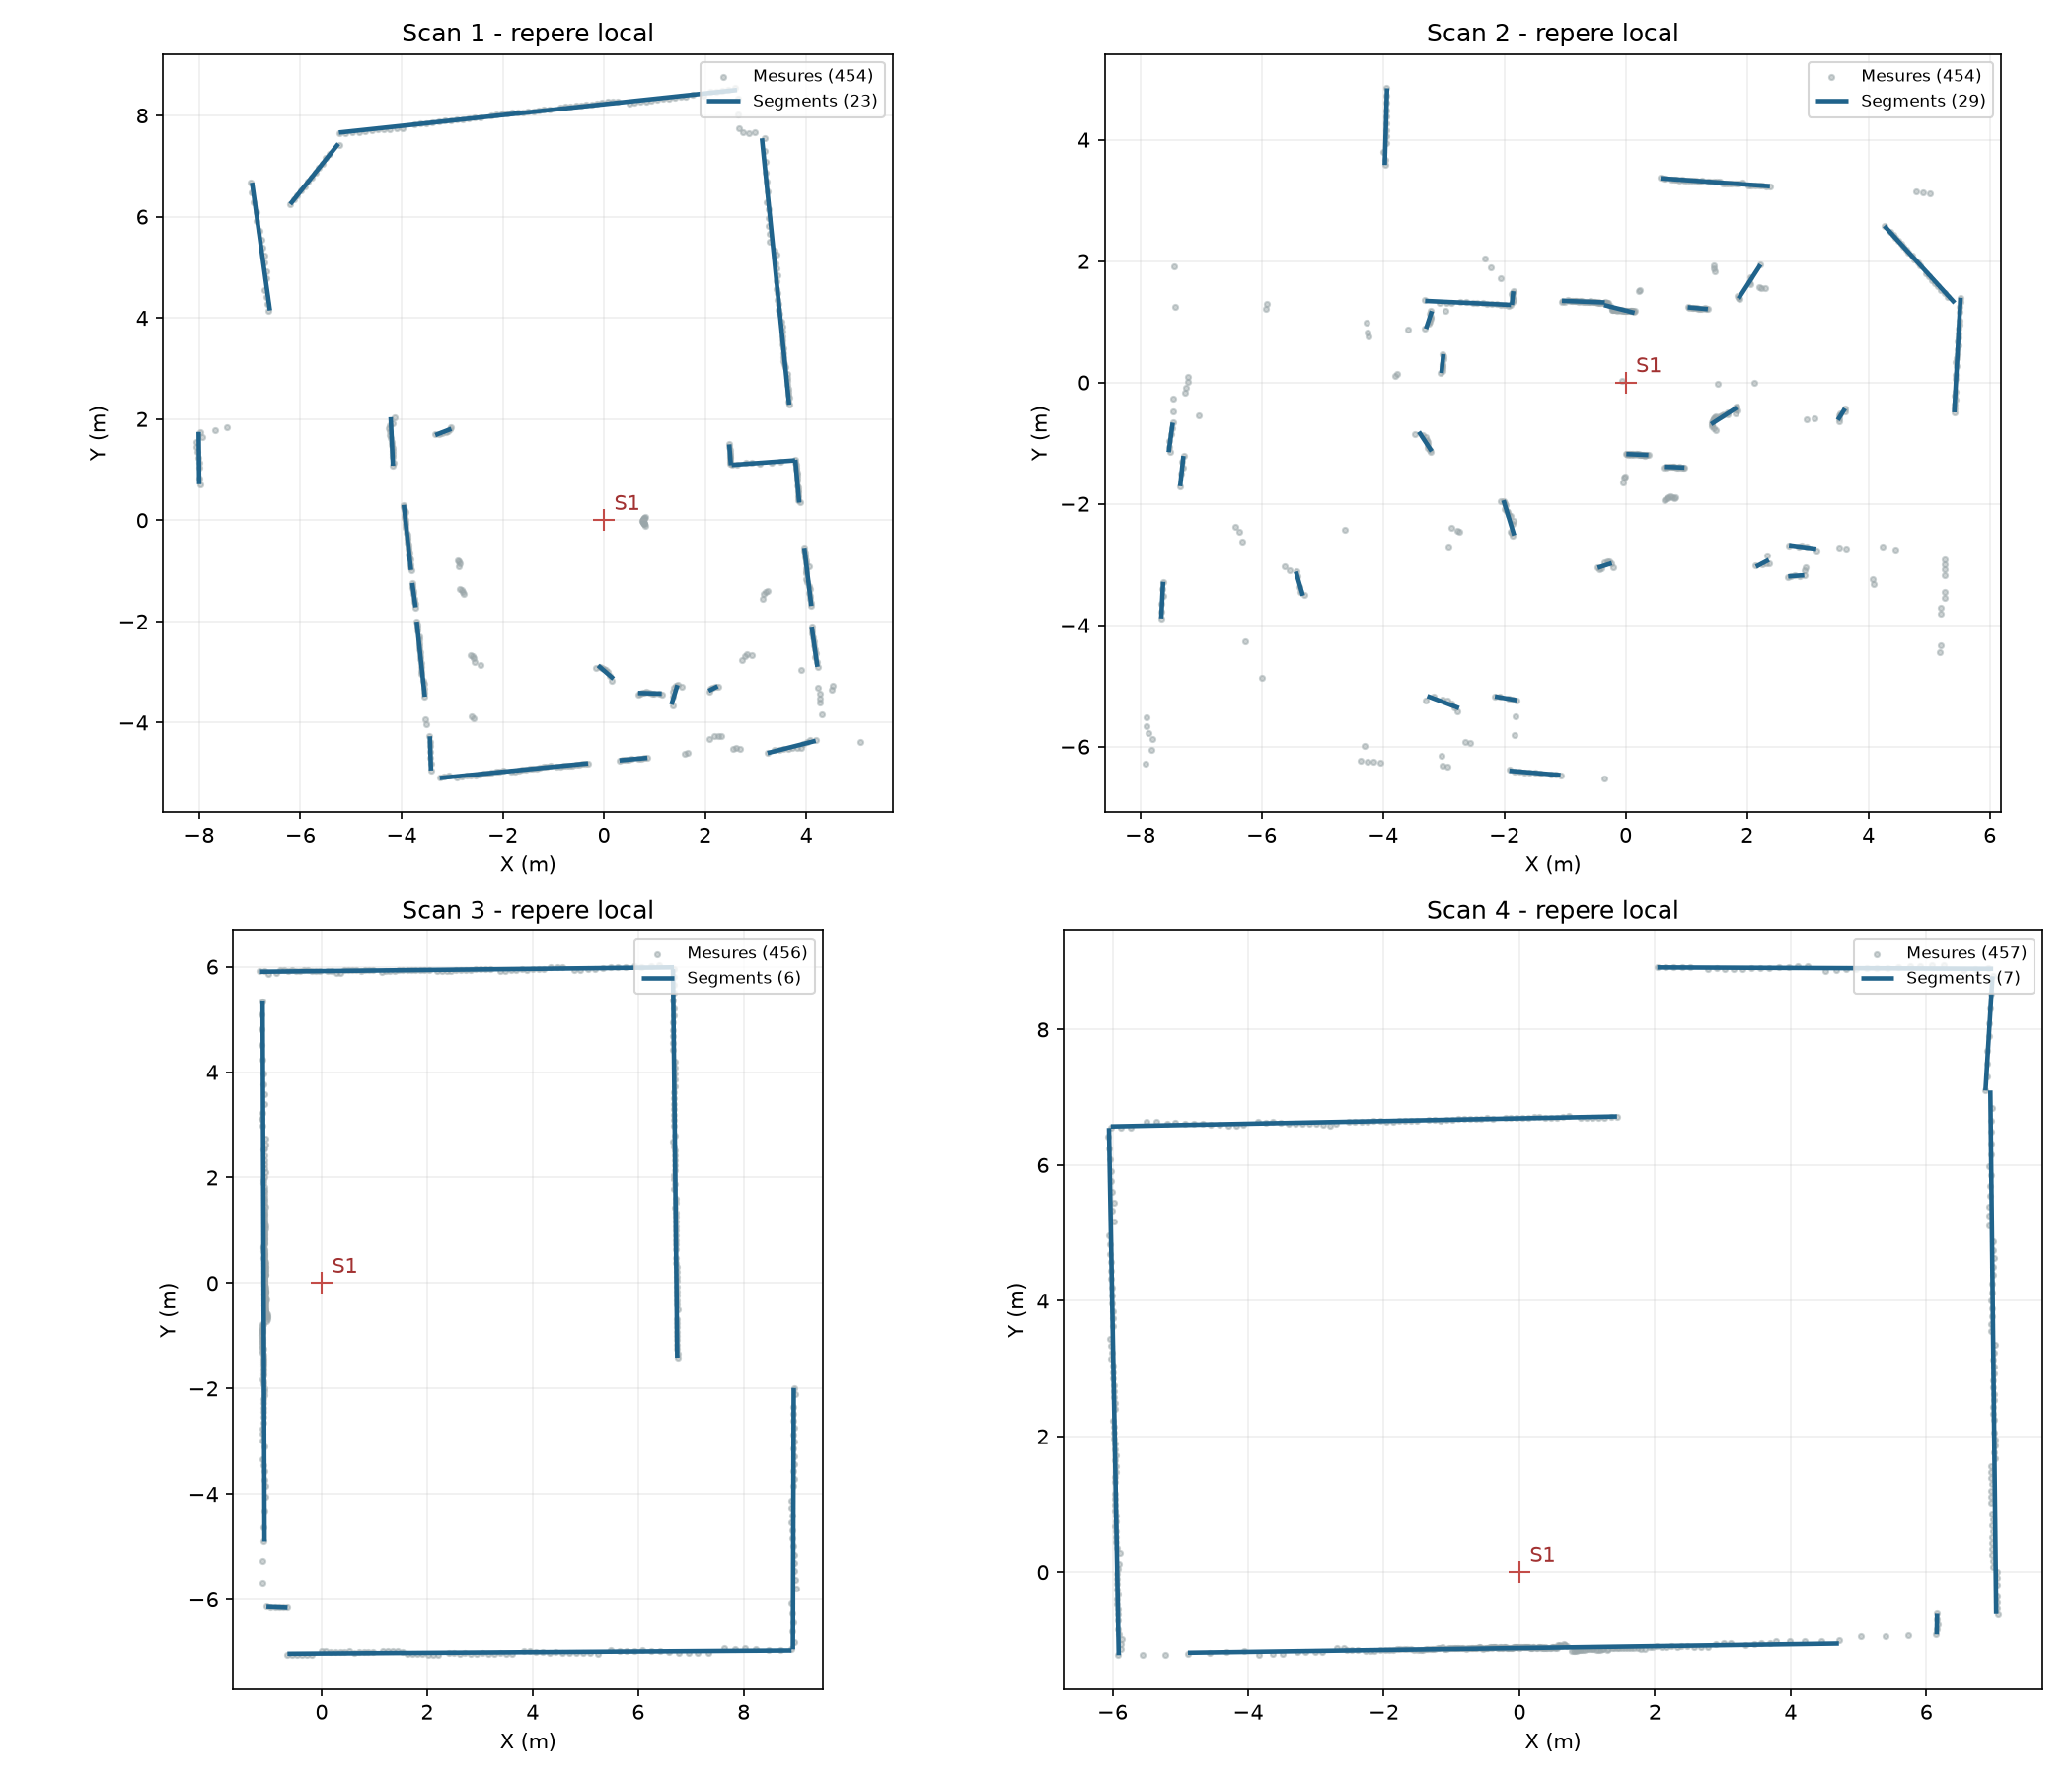
\includegraphics[width=\linewidth,height=.68\textheight,keepaspectratio]{vectorielles_individuelles.png}
\caption{Segments extraits séparément dans chaque repère local. Les mesures restent visibles pour contrôler l'ajustement.}
\end{figure}
\begin{figure}[H]\centering
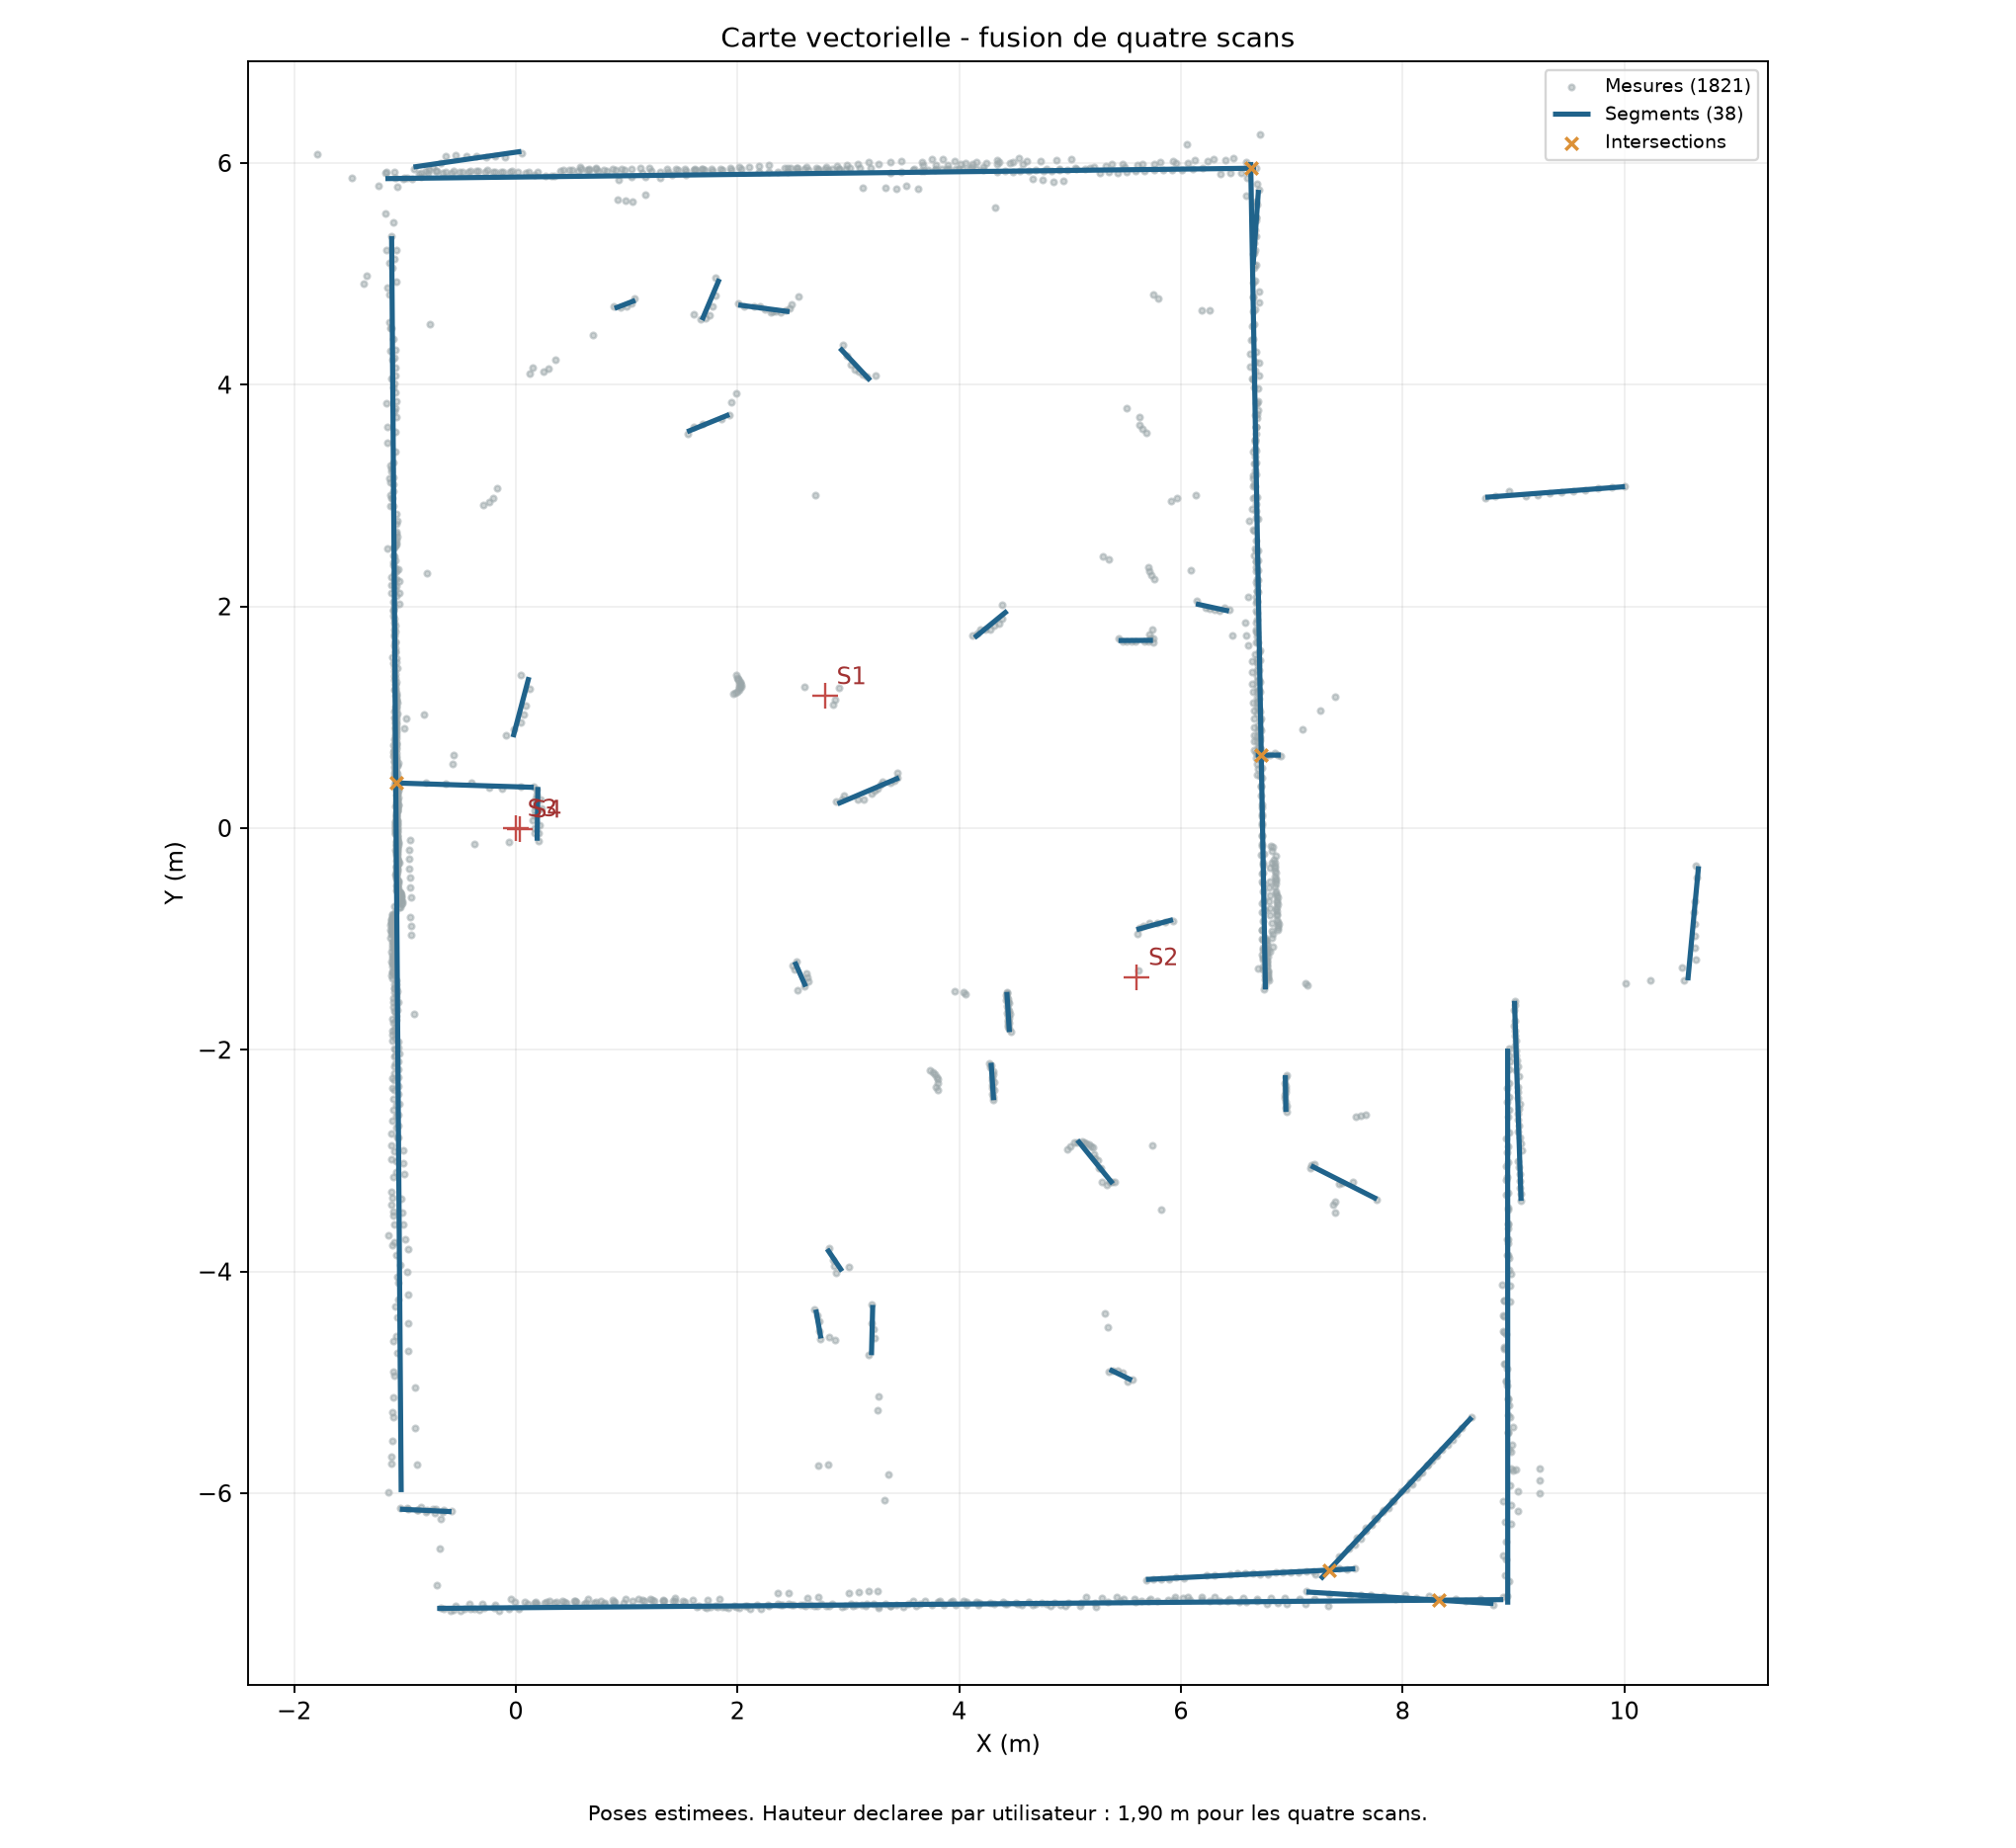
\includegraphics[width=.93\linewidth,height=.75\textheight,keepaspectratio]{carte_vectorielle.png}
\caption{Carte vectorielle fusionnée : mesures grises, segments bleus, intersections orange et origines estimées rouges.}
\end{figure}

\subsection{Lecture croisée des résultats}
Les trois figures finales répondent à des questions différentes. La fusion des nuages montre où les impacts ont été mesurés ; la grid map ajoute l'information sur les cellules effectivement traversées par les rayons ; la carte vectorielle résume les alignements suffisamment droits par des segments. Une zone blanche ou inconnue sur la grille ne devient pas libre parce qu'aucun point n'y apparaît dans le nuage. Inversement, un segment peut représenter plusieurs impacts proches sans indiquer l'épaisseur réelle d'un mur.
Le scan 4 se superpose fortement au scan 3 selon le critère de voisinage du tableau, tandis que le scan 2 se recale moins bien. Ainsi, les détails supplémentaires apportés par le scan 2 doivent être examinés avec prudence dans les deux cartes. Les 38 segments consolidés décrivent les structures détectées à la hauteur du capteur, pas un plan architectural certifié de la salle.

\section{Validation, fichiers livrés et limites}
Les 21 tests automatiques vérifient la géométrie, les cas limites de découpage, le tracé des rayons dans plusieurs directions, les conflits d'occupation, les indices négatifs, le rechargement d'une grille, la sélection des scans, les curseurs et les exports du viewer. Les callbacks sont testés sans fenêtre : cela ne remplace pas le contrôle visuel sur le poste de présentation.
Les exports ont également été contrôlés : 1\,821 lignes de mesures, quatre scans identifiés, 38 segments et une grille mise à jour quatre fois.

\begin{itemize}
\item \path{TP1_4_scans/data/} : quatre CSV bruts.
\item \path{TP1_4_scans/poses.json} : poses estimées, modifiables manuellement.
\item \path{TP1_4_scans/resultats/} : images, CSV individuels et fusionnés, grilles NPZ et métadonnées JSON.
\item \path{LD06_Atelier/} : code de lecture, visualisation, grilles, segments, recalage et tests.
\end{itemize}
Les limites principales sont l'absence de vérité terrain sur les poses, l'alignement moins cohérent du scan 2, les changements de scène et les zones masquées. La hauteur déclarée ne suffit pas à vérifier l'horizontalité. Aucune interpolation n'invente de surfaces pour fermer la pièce. Aucun lissage, vieillissement probabiliste ni SLAM complet n'est revendiqué. Ces cartes décrivent les surfaces observées à la hauteur de prise ; elles ne garantissent pas un passage libre pour un robot au sol.

\section{Reproduction et conclusion}
Depuis la racine du dépôt :
\begin{verbatim}
python -m pip install -r LD06_Atelier/requirements.txt
python TP1_4_scans/generer.py
python -m unittest discover -s LD06_Atelier -p "test_*.py" -v
\end{verbatim}
Les trois lanceurs Windows de \path{TP1_4_scans/} ouvrent les quatre nuages, la carte vectorielle ou la grille. Pour recalculer les poses, utiliser \path{TP1_4_scans/recaler.py} avant la génération.
Les cinq composantes du TP sont couvertes : données réelles, affichage multi-scans et réglage des poses, carte d'occupation mise à jour, géométrie des segments et carte vectorielle. La validation métrique de la pièce reste distincte de la validation du programme. Une mesure des poses et des acquisitions répétées dans des conditions contrôlées permettraient de renforcer le résultat avant une évaluation de localisation au TP2.

\begin{thebibliography}{9}
\bibitem{tp} Consigne du TP -- Jour 1, \emph{Extraction, Visualisation et Cartographie}, fournie par l'étudiant.
\bibitem{grid} Jonathan Quillès, \emph{Construction d'une grid map 2D à partir d'un scan LIDAR}, module Cartographie et Localisation, 2026, document fourni.
\bibitem{vector} Jonathan Quillès, \emph{Construction d'une carte vectorielle 2D à partir d'un scan lidar}, 2026, document fourni.
\end{thebibliography}
\end{document}
